% Auteur : Steve Prud’Homme
% Cette oeuvre, création, site ou texte est sous licence Creative Commons Attribution - Pas d’Utilisation Commerciale - Partage dans les Mêmes Conditions 4.0 International. Pour accéder à une copie de cette licence, merci de vous rendre à l'adresse suivante 
% http://creativecommons.org/licenses/by-nc-sa/4.0/ ou envoyez un courrier à 
% Creative Commons, 444 Castro Street, Suite 900, Mountain View, California, 94041, USA.

% :::SNIPET
% ::: SECTION
% \section{Contexte} 
%		\begin{frame}[allowframebreaks]
%			\frametitle{}
%			\begin {itemize}
%				\item 
%			\end{itemize}
%		\end{frame}
%:::WATER MARK / FILIGRANE
%\usepackage{draftwatermark}
%\SetWatermarkLightness{0.5}
%\SetWatermarkAngle{25}
%\SetWatermarkScale{0.5}
%\SetWatermarkFontSize{2cm}
%\SetWatermarkText{Document de travail}


\documentclass{beamer}
\usepackage{color}
\usepackage{beamerthemesplit} % new 
\usepackage[french]{babel}
\usepackage[utf8]{inputenc}
\usepackage{tikz}
\usepackage[fixlanguage]{babelbib}
\selectbiblanguage{french}
% Natlib pour la bibliographie
\usepackage{natbib}
\usepackage{url}
\usetikzlibrary{mindmap,shadows,shapes,backgrounds}
\usepackage[T1]{fontenc}
\setbeamertemplate{bibliography item}[text]
\usepackage{multicol}


\definecolor{MightySlate}{RGB}{85,98,112}
\definecolor{Pacifica}{RGB}{78,205,196}
\definecolor{AppleChic}{RGB}{199,244,100}
\definecolor{CheeryPink}{RGB}{255,107,107}

\setbeamercolor{titlelike}{parent=structure}
\setbeamerfont*{title}{size=\huge}
\setbeamercolor{title}{bg=MightySlate, fg=white}
\setbeamercolor{author}{bg=Pacifica, fg=white}
\setbeamercolor{institute}{bg=AppleChic, fg=black}
\setbeamercolor{date}{bg=CheeryPink, fg=white}

\definecolor{DTUred}{RGB}{178,20,20}
\setbeamercolor*{palette primary}{use=structure,fg=white,bg=MightySlate}
\usepackage{helvet}
\usepackage{draftwatermark}
\SetWatermarkLightness{0.5}
\SetWatermarkAngle{25}
\SetWatermarkScale{0.5}
\SetWatermarkFontSize{2cm}
\SetWatermarkText{Document de travail}

\begin{document}
	\title{Survol des situations de travail, des processus de production, du contrôle de la qualité et des bonnes pratiques en conception et réalisation d’outils pédagogiques en ligne} 
	\author{Steve Prud'Homme} 
	\institute{GTN-Québec - Commission scolaire de Laval} 
	\date{\today} 

	
	%\usebackgroundtemplate{%
  %\includegraphics[width=\paperwidth,height=\paperheight]{sommaire.png}} 
	
	\frame{\titlepage} 
	\usebackgroundtemplate{ } 
	\section{Sommaire} 
		\begin{frame}
			Cette présentation vise à :
			\frametitle{Sommaire}
			\begin {itemize}
				\item 
			\end{itemize}
		\end{frame}
	\frame[allowframebreaks]{\frametitle{Ordre du jour}\tableofcontents}


	\section{Introduction} 
		\begin{frame}[allowframebreaks]
			\frametitle{}
			\begin {itemize}
				\item 
			\end{itemize}
		\end{frame}
		
	\subsection{Présentation} 
		\begin{frame}[allowframebreaks]
			\frametitle{Présentation}
			\begin {itemize}
				
                                \item 2010-2013 : enseignant au DEP em  infographie
                                \item 2013-2016 : Travail au sein d’une équipe de production d’outil pédagogique en ligne comme conseiller technopédagogique et comme intégrateur
                                \item 2013 : Pratique réflexive et de comparaison avec ce qui se fait déjà dans l’industrie d’arts graphiques
                                \item 2013 : Membre du GTN-Québec
                                \item 2014-2015 : Survol des situations de travail, des processus de production, du contrôle de la qualité et des bonnes pratiques en conception et réalisation d’un outil pédagogique en ligneProjet de   
			\end{itemize}
		\end{frame}
			
            \subsection{Objectifs de la présentation} 
		\begin{frame}[allowframebreaks]
			\frametitle{Objectifs de la présentation}
			\begin {itemize}
				
                                \item La problématique
                                \item Cadre de référence
                                \item Méthodologie
                                \item Résultats
                                \item Suite ou interprétation
                        \end{itemize}
		\end{frame}

               \section{Problématique} 
		\begin{frame}[allowframebreaks]
			\frametitle{}
			\begin{itemize}
				\item 
			\end{itemize}
		\end{frame}

               \subsection{Contexte d'émergence} 
		\begin{frame}[allowframebreaks]
			\frametitle{Contexte d'émergence}
			\begin{itemize}
				\item Production de l'AEP en service de garde en ligne version 1
                                  \begin{itemize}
                                    \item L’équipe multidisciplinaire de production a vécu son lot de difficultés
                                    \item L’équipe de travail a été confrontée à un écart considérable entre le travail visé et la réalité de production.
                                    \item Cette réalité a amené l’équipe à porter une réflexion sur les pratiques dans le but de mieux comprendre ce qui ne fonctionnait pas dans son processus de production.
                                  \end{itemize}
                                \framebreak
                                \item Le défi de la version 2 de l'AEP service de garde en ligne
                                  \begin{itemize}
                                  \item Guider l’équipe de travail et les membres de la direction vers de nouvelles pratiques
                                  \item Faire preuve de tact avec l’équipe de travail et les membres de la direction afin de les amener à une réflexion sur leurs pratiques. 
                                  \item Production d'un premier document intitulé : « Projet de flux de production d’un projet de cours en ligne » 
                                    \begin{itemize}
                                      \item Ce document traite des balises et limites d’un tel flux de production pour un projet de cours en ligne et ses constituantes
                                      \item Ce flux de production inclut inclut les tâches, les livrables et les points de contrôles, tout en définissant les principaux concepts liés, les matériaux d’un projet de cours en ligne.
                                         
                                    \end{itemize} 
                                  \end{itemize}                                             
                                \end{itemize} 
                        \end{frame}

  \subsection{Contexte d'application} 
		\begin{frame}[allowframebreaks]
			\frametitle{Contexte d'application}
			Plusieurs écrits documentent la conception d’outil pédagogique en ligne, mais le point de vue des auteures ou des auteurs diverge sur les différentes étapes nécessaires à leur réalisation \citep[p.18]{bonneau2013a}.
                   \begin{figure}
                     \centering
                     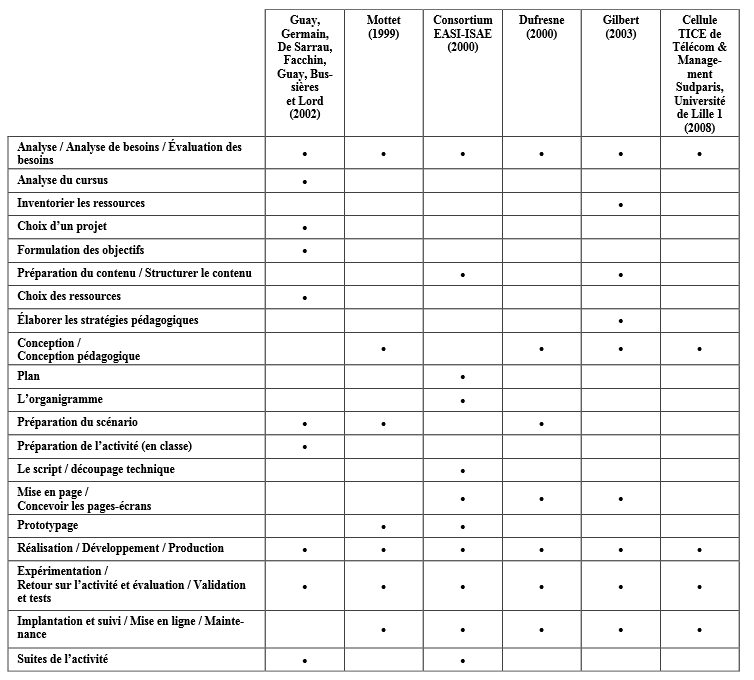
\includegraphics[width = 0.52\textwidth]{tableau6methodes.png}
                     \caption{\tiny{Tableau comparatif des étapes de six méthodes utilisées pour la conception et la réalisation d’outils pédagogiques en ligne \citep[p.20]{bonneau2013a}}}
                   \end{figure}
                   \begin{itemize}                   
                   \item On constate donc qu’il y a une grande disparité entre les méthodes et que, comme le dit \citet{bonneau2013a} , peu font l’unanimité. 
                   \item La variété des méthodes pourrait s’expliquer par le fait que les outils pédagogiques en ligne sont protéiformes, c’est-à-dire qui peut prendre diverses formes.
                   \item Il faut donc demeurer critiques sur l’application d’un processus systématique
                   \item \citet[p.10]{retalis1997a}, \citet[p.46]{smith2006a} et \citet[p.3]{pohl2004a} le confirment.
                   \end{itemize}
			\par \citet[p.3]{pohl2004a} prétend que : 
			\par« Guidelines for the development of e-learning systems have advantages and disadvantages. One disadvantage is that it is sometimes difficult to generalize guidelines. Related to that is the fact that the efficiency of educational media always depends on the context in which they are used. Guidelines should, therefore, not be formulated as cookbook recipes but rather be flexible tools which can be adapted to various different situations and environments. If such a flexible approach is used, guidelines can be applied quite effectively ».
			\par  Il a donc fallu prévoir, lors du survol, traiter de l’aspect de la situation de travail: soit du contexte dans le cadre duquel les processus sont utilisés.
                \end{frame}

\subsection{Milieu et les personnes concernées} 
		\begin{frame}[allowframebreaks]
			\frametitle{Précision sur le milieu et les personnes concernées}
                        \
                        \begin{itemize} 
                        \item  Les équipes sont multidisciplinaires ;
                        \item Composées de spécialistes des contenus qui peuvent être des enseignants, des spécialistes de la formation ou des conseillers pédagogiques ;
                        \item Ces équipes sont formées de : 
                        	\begin{itemize}
                        		\item concepteur pédagogique / conseillers pédagogiques ou technopédagogiques,
                        		\item intégrateurs, les infographistes, les programmeurs, les spécialistes des réseaux,
                        		\item de chargés de projets ou gestionnaires dirigent les projets.
                        	\end{itemize}

                        \end{itemize}

             
                \end{frame}

\subsection{La nécessité} 
		\begin{frame}[allowframebreaks]
			\frametitle{La nécessité d’un survol}
                        
                        \begin{itemize} 
                        \item  Les méthodes dans le domaine de la conception et de la réalisation d’outils pédagogiques en ligne sont importantes \citep[p. 842]{bohl2002a}, \citep[p. 218]{barry2003a}, \citep[p. 1]{hadjerrouit2007a} tirés de \cite{bonneau2013a};
                        \item La conception et la réalisation d’outils pédagogiques en ligne sont souvent faites par des novices en la matière \citep[p. 351]{verstegen2008a} tiré de \citet{bonneau2013a};
                        \item Les enseignants semblent avoir une vision restreinte au niveau de l’ampleur et de la complexité (voire l’entièreté des problèmes) que l’appropriation d’une telle pratique peut créer, soit une vision générale de tout le processus engendré par une telle démarche dans un dispositif de FAD \citep[p. 105]{roy2011a} tiré de \citet{bonneau2013a}; 
                        \item Les méthodes d’ingénierie pédagogique comme la méthode ADDIE,aurais provoqué une simplification de la perception qu’ont de nombreux acteurs du domaine de l’éducation de ce processus\citep[p.28]{bonneau2013a}. 

                        \end{itemize}

             
                \end{frame}


\section{Bibliographie}
\subsection{Bibliographie}
\frame[allowframebreaks]{\frametitle{Bibliographie}

\bibliographystyle{apalike}
\bibliography{bibliographie} %bibtex file name without .bib extension
}
\end{document}

